\documentclass{beamer}
%
% Choose how your presentation looks.
%
% For more themes, color themes and font themes, see:
% http://deic.uab.es/~iblanes/beamer_gallery/index_by_theme.html
%
\mode<presentation>
{
  \usetheme{Boadilla}      % or try Darmstadt, Madrid, Warsaw, ...
  \usecolortheme{beaver} % or try albatross, beaver, crane, ...
  \usefonttheme{default}  % or try serif, structurebold, ...
  \setbeamertemplate{navigation symbols}{}
  \setbeamertemplate{caption}[numbered]
  
} 

\usepackage{xcolor,colortbl}
\usepackage[english]{babel}
\usepackage[utf8x]{inputenc}
\usepackage{courier}
\usepackage{dsfont}
\usepackage{verbatim} 
\usepackage{enumerate}
\usepackage{tikz}
\usepackage{multirow}
\usepackage{venndiagram}
\usepackage{epigraph} 
%\usepackage{xcolor}
\usepackage{makecell}

%\usepackage{enumitem}

\usepackage{hyperref}
\hypersetup{
    colorlinks=true,
    linkcolor=blue,
    filecolor=magenta,      
    urlcolor=cyan,
}

% R stuff!
\usepackage{listings}
\definecolor{codegreen}{rgb}{0,0.6,0}
\definecolor{codegray}{rgb}{0.5,0.5,0.5}
\definecolor{codepurple}{rgb}{0.58,0,0.82}
\definecolor{backcolour}{rgb}{0.95,0.95,0.92}

\lstdefinestyle{mystyle}{
    backgroundcolor=\color{backcolour},    
    commentstyle=\color{codegreen},
    keywordstyle=\color{black},
    numberstyle=\tiny\color{codegray},
    stringstyle=\color{codepurple},
    basicstyle=\ttfamily\footnotesize,
    breakatwhitespace=false,         
    breaklines=true,                 
    captionpos=b,                    
    keepspaces=true,                 
    numbers=left,                    
    numbersep=5pt,                  
    showspaces=false,                
    showstringspaces=false,
    showtabs=false,                  
    tabsize=2
}

\lstset{style=mystyle}


\setbeamertemplate{enumerate items}[default]
\setbeamertemplate{itemize item}[triangle]

%\setitemize{label=\usebeamerfont*{itemize item}%
%  \usebeamercolor[fg]{itemize item}
%  \usebeamertemplate{itemize item}}



\title[SST-115 / STA-209]{Odds and Risk}
\subtitle{}
\author{Grinnell College}
\date{September 16, 2024}

\graphicspath{{img/}}

\begin{document}

\begin{frame}
  \titlepage
\end{frame}

\begin{frame}{Review}
Probabilities
\begin{itemize}
    \item Unions (possibility of either event)
    \item Intersections (2 events at same time)
    \begin{itemize}
        \item Disjoint (2 events \textit{can't} happen at same time)
    \end{itemize}
    \item Conditionals (one event has already happened)
    \begin{itemize}
        \item Independence (do conditions add extra info?) 
    \end{itemize} \vspace{4mm}
\end{itemize}
Lots of Probability math
\end{frame}

\begin{frame}{Outline for Today}
\begin{itemize}
\item Introduce odds (another likelihood comparison)
\item Odds ratios
\item Relative Risk
\end{itemize}
\end{frame}

\begin{frame}{Law of Large Numbers}
As our sample size increases, the empirical probability of something happening approaches the true probability (only holds when trials cannot influence each other)
\begin{center}
    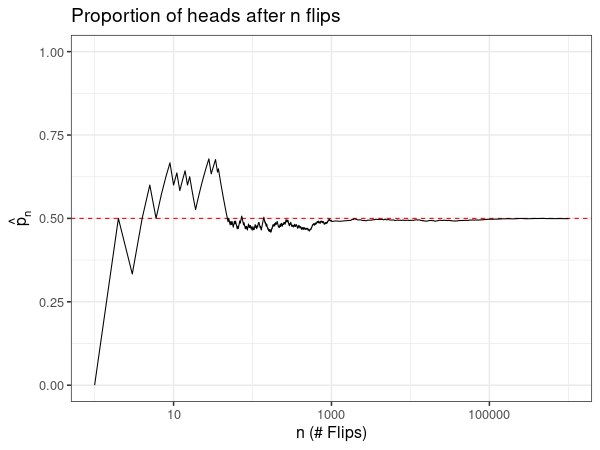
\includegraphics[scale=.4]{img/lln_flip.png}
\end{center}
\end{frame}



\begin{frame}{Odds and Probability}
When dealing with a \textit{binary} event, we often speak in terms of \textbf{odds}, a \textit{ratio} of ``number of successes" to ``number of failures"  \vspace{4mm}

\begin{align*}
\text{ \# success : \# failure}
\end{align*}

This is distinct from the idea of \textbf{probabilities}, which give a ratio of the ``number of successes" to the number of possible outcomes

\begin{align*}
\text{ \# success} &: \text{\# total outcomes} \\
&: \text{\# success + \# failure}
\end{align*}

\end{frame}


\begin{frame}{Odds}
Suppose we have a 6-sided die, and we are interested in rolls that land on either 1 or 2 (note how we have turned six distinct outcomes into two ``events").

\begin{align*}
\text{Die} = \{ \color{red} 1, 2 \color{black}, 3, 4, 5, 6 \}
\end{align*}

\begin{itemize}
\item The \textit{probability} of rolling a 1 or 2 is 1/3
\begin{enumerate}
\item There are 6 possible outcomes
\item There are 2 possible successes
\item Probability is 2/6 = 1/3
\end{enumerate} \vspace{2mm}
\item The \textit{odds} of rolling a 1 or 2 are 2:4 (or 1:2)
\begin{enumerate}
\item There are 2 possible successes
\item There are 4 possible failures
\item The odds of success are 2:4 (or 1:2)
\end{enumerate}
\end{itemize}

\end{frame}





\begin{frame}{Odds Examples}

The order of the event and non-event in this table matters for our calculations:

\begin{table}[ht]
\centering
\begin{tabular}{|r|r|r|}
  \hline
 & Event & Non-Event \\ 
  \hline
Exposure & A & B \\ \hline
No Exposure & C & D \\
   \hline
\end{tabular}
\end{table}

\begin{itemize}
\item The odds of an event for the exposure group are A:B (or A/B)
\item The odds of an event for the no exposure group are C:D (or C/D)
\end{itemize}

\vspace{6mm}
The \textbf{odds ratio} for these groups is then the ratio of their odds:

\begin{align*}
OR &= \frac{A:B}{C:D} = \frac{A/B}{C/D} = \frac{A \times D}{B \times C}
\end{align*}

\end{frame}


\begin{frame}{Why Ratios?}

Situation 1:
\begin{table}[ht]
\centering
\begin{tabular}{|r|r|r|}
  \hline
 & Event & Non-Event  \\ 
  \hline
Exposure & 6 & 2  \\ \hline
No Exposure & 3 & 2  \\
   \hline
\end{tabular}
\end{table}

Situation 2:
\begin{table}[ht]
\centering
\begin{tabular}{|r|r|r|}
  \hline
 & Event & Non-Event \\ 
  \hline
Exposure & 103 & 2 \\ \hline
No Exposure & 100 & 2 \\
   \hline
\end{tabular}
\end{table}

\begin{enumerate}
\item Difference in odds for each situation?
\item Ratio of odds for each situation?
\end{enumerate}

\end{frame}

\begin{frame}{Event vs Non-Event}

Which column is our ``Event" changes how we report our results \\ \vspace{4mm}

Case 1: 
\begin{table}[ht]
\centering
\begin{tabular}{|r|r|r|}
  \hline
 & Survive & Death \\ 
  \hline
Treatment & 12 & 6 \\ \hline
Placebo & 5  & 10 \\
   \hline
\end{tabular}
\end{table}

Case 2: 
\begin{table}[ht]
\centering
\begin{tabular}{|r|r|r|}
  \hline
 & Death & Survive \\ 
  \hline
Treatment & 6 & 12 \\ \hline
Placebo & 10  & 5 \\
   \hline
\end{tabular}
\end{table}
\end{frame}

\begin{frame}{Group Rows}

The same is true for which group is in the first row \\ \vspace{4mm}

Case 1: 
\begin{table}[ht]
\centering
\begin{tabular}{|r|r|r|}
  \hline
 & Survive & Death \\ 
  \hline
Treatment & 12 & 6 \\ \hline
Placebo & 5  & 10 \\
   \hline
\end{tabular}
\end{table}

Case 2: 
\begin{table}[ht]
\centering
\begin{tabular}{|r|r|r|}
  \hline
 & Survive & Death \\ 
  \hline
Placebo & 5  & 10 \\ \hline
Treatment & 12 & 6 \\
   \hline
\end{tabular}
\end{table}
\end{frame}


\begin{frame}{Odds Ratio Summary}

\begin{itemize}
\item Odds and probabilities 
\item Column/row order matters
\item Odds ratios
\item $OR > 1$, $OR = 1$, $OR < 1$
\begin{itemize}
\item $OR = 1$ implies no association. Why?
\end{itemize}
\end{itemize}


\end{frame}


\begin{frame}{Example 1} 

{\scriptsize A report published in 1988 summarizes results of a Harvard Medical School clinical trial determining effectiveness of asprin in preventing heart attacks in middle-aged male physicians}

\begin{center}
\begin{tabular}{|p{3cm}|p{3cm}|p{3cm}|}
\hline
 & \multicolumn{2}{c|}{Myocardial Infarction}      \\ \cline{2-3}
  Treatment Status   & Attack & No Attack      \\ \hline
  Placebo  & 189  & 10,845   \\ \hline
  Asprin & 104   & 10,933   \\ \hline
% Total  & $40$ & $60$ & $100$ \\ \hline
\end{tabular}
\end{center}

\begin{itemize}
\item Odds of having a heart attack for placebo: 
\item Odds ratio for treatment and infarction:
\item Associated?
\end{itemize}

\end{frame}

\begin{frame}{Example 2}

{\scriptsize The table below shows the results for drivers and passengers in auto accidents in Florida in 2008, according to whether or not the individual was wearing a seat belt.}

\begin{center}
\begin{tabular}{|p{3cm}|p{3cm}|p{3cm}|}
\hline
 & \multicolumn{2}{c|}{Injury}      \\ \cline{2-3}
  Sealt-Belt Use   & Fatal & Nonfatal      \\ \hline
  No  & 1085  & 55,623   \\ \hline
  Yes & 703   & 441,239  \\ \hline
% Total  & $40$ & $60$ & $100$ \\ \hline
\end{tabular}
\end{center}

\begin{itemize}
\item \textit{Probability} of wearing seatbelt conditional on fatality status:
\item \textit{Odds} of fatality conditional on seat-belt use: 
\item Associated?
\end{itemize}
\end{frame}

\begin{frame}{Relative Risk}
Just like looking at odds ratios, we can look at probability ratios. These are often called \textbf{relative risk}.
\begin{itemize}
    \item again, the order of events matters
\end{itemize}

\begin{center}
\begin{tabular}{|p{3cm}|p{3cm}|p{3cm}|}
\hline
 & \multicolumn{2}{c|}{Injury}      \\ \cline{2-3}
  Sealt-Belt Use   & Fatal & Nonfatal      \\ \hline
  No  & 1085  & 55,623   \\ \hline
  Yes & 703   & 441,239  \\ \hline
% Total  & $40$ & $60$ & $100$ \\ \hline
\end{tabular}
\end{center} \vspace{3mm}

relative risk of fatality for no-seat-belt use: \vspace{2mm}

$\frac{\textbf{P(Fatality if Seat-Belt Use = No)}}{\textbf{P(Fatality if Seat-Belt Use = Yes)}}$ =  $\frac{1085 / (1085 + 55623)}{703 / (703 + 441239)}$ = 12.02
\begin{itemize}
    \item Prob. of Fatality is roughly 12 times \textit{higher } for the no-seat-belt group
\end{itemize} \vspace{2mm}

relative risk of fatality for seat-belt use: \vspace{2mm}

$\frac{\textbf{P(Fatality if Seat-Belt Use = Yes)}}{\textbf{P(Fatality if Seat-Belt Use = No)}}$ =  $\frac{703 / (703 + 441239)}{1085 / (1085 + 55623)}$ = .083
\begin{itemize}
    \item Prob. of Fatality is .083 times \textit{less} for the seat-belt group
\end{itemize}
\end{frame}

%\begin{frame}[fragile]
%\tiny
%\begin{lstlisting}[language=R]
%ggplot(majors, aes(x = Per_Male, y = Bach_Med_Income)) + 
%  geom_point() 
%\end{lstlisting}
%\vspace{2mm}
%
%\end{frame}


%%%%%%%%%%%%%%%%

%\begin{frame}
%\begin{columns}
%
%  \begin{column}{0.45\textwidth}
%%
%  \end{column}
%  \begin{column}{0.45\textwidth}
%%
%  \end{column}
%
%\end{columns}
%\end{frame}


\end{document}
